%PIP-412029OA046
\documentclass[reprint,amsmath,amssymb,aps,prb,footinbib,floatfix]{revtex4-2}
\bibliographystyle{apsrev4-2}
\usepackage{afterpage}
\usepackage{blindtext}
\usepackage[rgb]{xcolor}
%\usepackage[twocolumn=true,includehead=false,left=.75in,right=.75in,top=.75in,bottom=.75in]{geometry}
%\usepackage[letterpaper, portrait, twocolumn, twoside, left=2cm, hmarginratio=2:1, includemp, marginparwidth=43pt, bottom=1cm, foot=.7cm, includefoot, textheight=11cm, heightrounded, columnsep=1cm, dvips, verbose]{geometry}
\definecolor{Cred}{RGB}{208, 32, 46}
\usepackage[firstpage=true]{background}
\usetikzlibrary{calc}
%\usepackage{tikz}
\backgroundsetup{angle = 0, scale = 1, vshift = 0pt, opacity=1,
  contents = {\begin{tikzpicture}[overlay,remember picture]
    \node at (0,0) {\includegraphics[scale=1]{EC_RC.pdf}};
\end{tikzpicture}
}
}
%    \draw (3.4in,3.75in) node[inner sep=0] {\includegraphics[width=1in]{arrow.pdf}};
%    \draw (3.5in,3.85in) node[rotate=-90] {\scshape{Editor's}};
%    \draw (3.5in-\baselineskip,3.85in) node[rotate=-90] {\scshape{Suggestion}};
%\end{tikzpicture}

\usepackage{graphicx} % Required for inserting images
\usepackage{mathtools} % Useful for a bunch of math stuff
\usepackage{cleveref} % Use for better cross-references
\usepackage[caption=false]{subfig} % For sub-figures
\usepackage{booktabs} % For nicer looking tables
\usepackage[twoside]{fancyhdr}
\usepackage{appendix}

\usepackage{placeins}




\fancypagestyle{plain}{%
%\setlength{\headheight}{60pt}
\fancyhead[L,C]{}
\fancyhf{}
\fancyhead[R]{\raisebox{.6cm+1pt}{\textbf{Rapid Communication}}}
\fancyhead[L]{ \raisebox{.6cm+1pt}{\scshape{Editor's Suggestion}\vspace{12pt}}}
\fancyhead[C]{\raisebox{.6cm}{\large\scshape{CARTHAGE}}\hspace{0.2cm}\includegraphics[height=1.5cm]{Logo.pdf}\hspace{0.1cm}\raisebox{.6cm}{\large\scshape{COLLEGE 
 }}}
\fancyfoot[C]{\thepage}
\renewcommand{\headrulewidth}{0pt}
\renewcommand{\footrulewidth}{0pt}
}
\usepackage{printlen}


\pagestyle{fancy}
\fancyhf{}
\fancyheadinit{\setlength{\headheight}{20pt}}
\fancyhead[RO,LE]{\textbf{Rapid Communication}}
\fancyhead[LO,RE]{\textit{Phys. in Prog.} \textbf{2} (Feb. 2026)}
\fancyhead[C]{ \large \scshape{PHYSICS IN PROGRESS}}
\fancyfoot[C]{\thepage}
\renewcommand{\headrulewidth}{0.4pt}
\renewcommand{\footrulewidth}{0pt}

% These are packages I am using in this document
\usepackage{siunitx}

% Everything up to here is the 'document preamble'

\begin{document} 

\vspace*{25pt}


\title{Estimating Planck's constant using the photoelectric effect}% Force line breaks with \\


\author{Sema'Je Zechariah Farmer}
\affiliation{%
Department of Physics and Astronomy,  Carthage College, 2001 Alford Park Drive, Kenosha, WI 53140, USA
}%
\collaboration{Received January 29, 2026, Published online February 5, 2026}

\begin{abstract}

The photoelectric effect occurs when light of a sufficiently high frequency strikes a surface, exciting the electrons on that surface to the point that they are ejected from it. Those ejected electrons are called photoelectrons, which can be collected and sent through a circuit. By measuring the resulting current and the negative voltage required to stop it at various frequencies and intensities, some essential relationships can be established. The first is the relationship between stopping voltage and frequency. This relationship is linear, and using its slope, Planck’s constant was estimated to be 6.5(2) \(\times\) 10\(^{-34}\) Js. The second relationship is between the stopping voltage and intensity. Classical wave theory predicts that an increase in intensity should increase the stopping voltage. In reality, the data shows that the two are entirely unrelated. This result directly contradicts wave theory, supporting theories of light’s particle-like behavior and the existence of photons.



\end{abstract}

%\keywords{Suggested keywords}%Use showkeys class option if keyword
                              %display desired
\maketitle

%\tableofcontents

\section{\label{sec:level1} Introduction}

The debate on whether light behaves as waves or particles spanned multiple centuries. It began in the early 1600s with various theories on both sides of the argument, but concluded in the early 1900s with Einstein's explanation of the photoelectric effect \cite{Arons1965}. Heinrich Hertz originally discovered this effect \cite{Vesely2002}, and later Philipp Lenard studied it \cite{Wheaton1978} . Lenard used a carbon-arc light to excite electrons on a metal plate. Those excited electrons would then be ejected from that plate and collected on another plate located some distance away from the emitter. The collector plate was then connected to a cathode and a sensitive ammeter, allowing him to measure the current induced by the collected electrons. In his studies, Lenard compared the energy of the photoelectrons (ejected electrons) to the intensity of the light coming from the source. To measure the energy of the electrons, Lenard applied a negative charge to the collector plate, repelling any electrons that lacked sufficient energy to pass. In doing so, Lenard discovered a quantity called the stopping voltage, the voltage applied to the collector plate that prevents all electrons from reaching it. Through testing, Lenard found that this stopping voltage remained constant regardless of the source's light intensity  \cite{Fowler}. He even went so far as to test this with different colors, finding that the stopping voltage actually depends on the wavelength of light \cite{Fowler}. Einstein suggested that light radiation should be thought of as quanta called photons, each with energy $hf$, where each photon transfers its energy to a single electron.




\section{Theory}
In this experiment, we used the PASCO SE-6609 photoelectric effect apparatus to recreate Lenard's experiment. The apparatus uses a mercury lamp to illuminate a receiver. The receiver then filters out all but one wavelength of light. From there, the filtered light hits the emitter plate, ejecting electrons into the collector plate, and we measure the current induced by those electrons as seen in fig \ref{fig:Circuit}. 

\begin{figure}
    \centering
    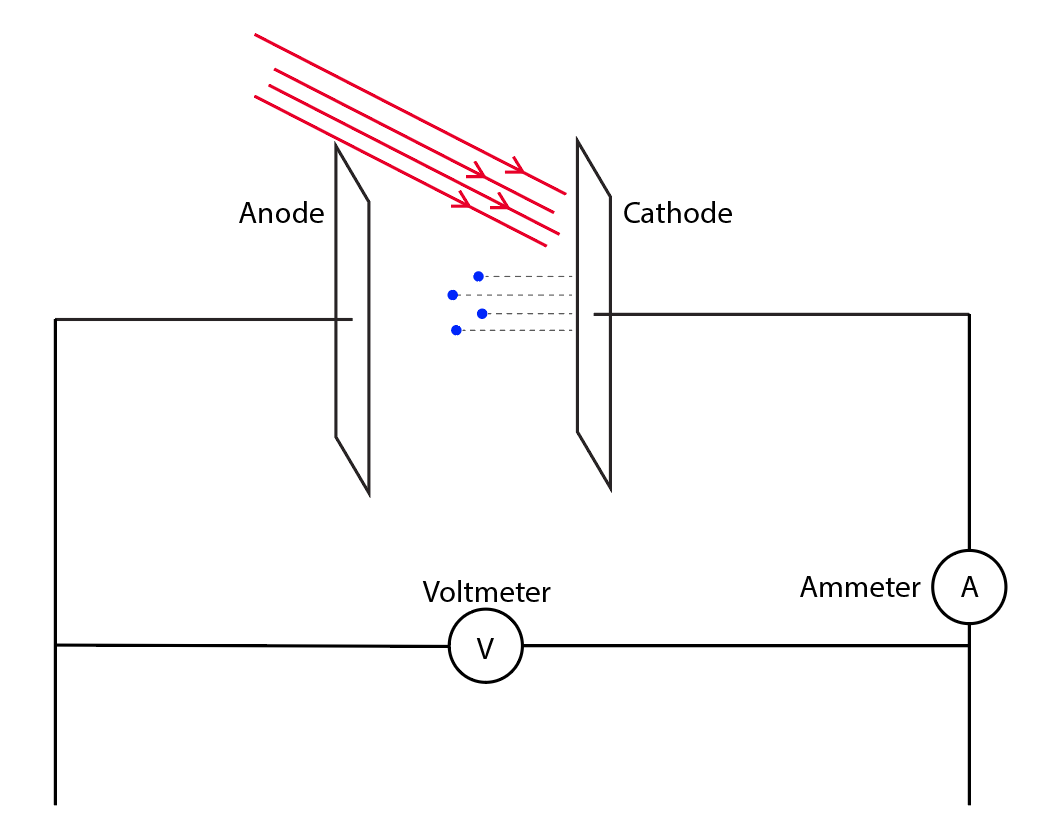
\includegraphics[width=1\linewidth]{Circuit.png}
    \caption{Basic circuit of the photoelectric effect. Light strikes the emitter plate on the right, exciting the electrons enough to eject them towards the collector plate on the right. An ammeter is included in the circuit to measure the induced current, and a voltmeter is included to measure the potential difference between the two plates.}
    \label{fig:Circuit}
\end{figure}


Similar to Lenard's experiment, we measure the current induced at different intensities and the stopping voltage at various frequencies. We then attempt to use that collected data to estimate Planck's constant and confirm Einstein's photon theory.

If the energy ($E$) of a photon is equal to Planck's constant ($h$) multiplied by the photon frequency ($f$), and that photon only transfers its energy into a single electron \cite{Arons1965}, then the energy of the ejected electron can be described by

\begin{equation}
    E=hf - \phi
    \label{E electron},
\end{equation}
where $\phi$ is the work function for the cathode. The work function represents the amount of work required to free electrons from a given material and, as such, is dependent on the material surface of the cathode. In the case of the PASCO apparatus used in this experiment, the material is likely a light-sensitive metal with a low work function.
The stopping voltage ($V_{stop}$) can be derived from eq. \ref{E electron} by substituting in $eV$ for the energy and solving for $V$.   

\begin{equation}
    V_{stop}=\frac{h}{e}f - \frac{\phi}{e}
    \label{Vstop}
\end{equation}

where $e$ is the charge of electrons. This equation shows a linear relationship between $V_{\text{stop}}$ and $f$. So a plot of $V_{\text{stop}}$ vs. $f$ should result in a slope of $h/e$ and a y-intercept of $\phi/e$. The goal of this experiment is to demonstrate the relationship with physical data that can then be used to estimate Planck's constant.



To do so, we collected two datasets. The first was stopping voltage vs intensity. This dataset was collected to verify that the stopping voltage is independent of light intensity. The stopping voltage was recorded by increasing the negative voltage applied until the current read zero. The lowest voltage magnitude at which the current stopped was recorded as the stopping voltage for that test. Intensity was not directly measured; instead, it was implied. It is well documented that the intensity of electromagnetic radiation decreases with increasing distance from the source to the receiver. This relationship is known as the inverse-square law \cite{BROWNSON2014}, which states that $I \propto r^ {-2}$ \cite{Krane19}. So changing $r$ (the distance) will inversely affect $I$ by a factor of $r^2$. With this in mind, the stopping voltage was measured at four different distances (and by translation intensities) for four different wavelengths.
The second data set was the stopping voltage vs frequency. This was collected to both establish that stopping voltage depends on frequency and to estimate Planck's constant. The stopping voltage we measured using the same methodology as the other data set, and the frequency is given by the selected wavelength.

Measurements of stopping voltage vs intensity yielded the expected results. It was hypothesized that the stopping voltage at a given frequency should remain constant regardless of light intensity. So we'd expect $V_{\text{stop}}$ to stay the same for any distance.

\begin{figure}
    \centering
    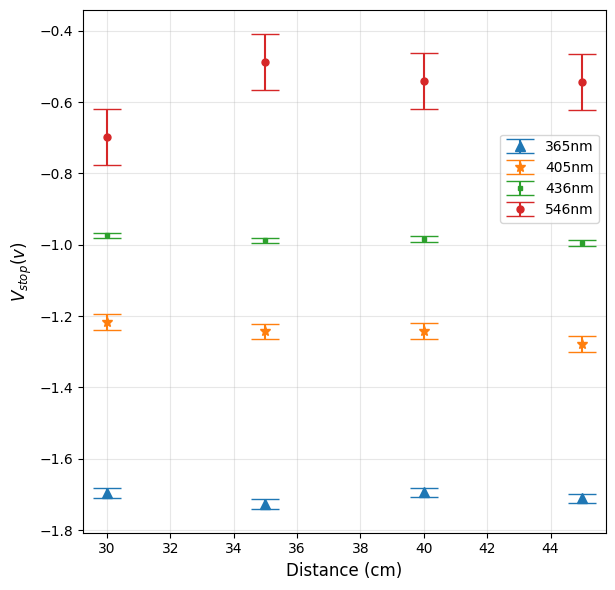
\includegraphics[width=0.8 \linewidth]{Dist2.png}
    \caption{Stopping voltage versus distance scatter plot. Measuring the stopping voltage at various distances for four different wavelengths of light.}
    \label{fig:Distance}
\end{figure}

 Fig. \ref{fig:Distance} shows the results of data collection for all four wavelengths. For all four wavelengths, a hypothesis test was conducted to determine how far each $V_{\text{stop}}$ is from the mean in its series. The result of this analysis was good across the board, with Z scores across all series remaining just at or below $\pm0.75$. This indicates a high level of consistency and no significant deviation from the mean. The fact that the measurements taken for the stopping voltage at each wavelength remain mostly constant shows that the stopping voltage is not dependent on the intensity of light. This result directly contradicts the wave theory and supports the particle theory of light. 

 Data collection and analysis on stopping voltage vs. frequency was just as successful. Based on eq.\ref{Vstop} we expect physical results to show a linear relationship between stopping voltage and frequency.

\begin{figure}
    \centering
    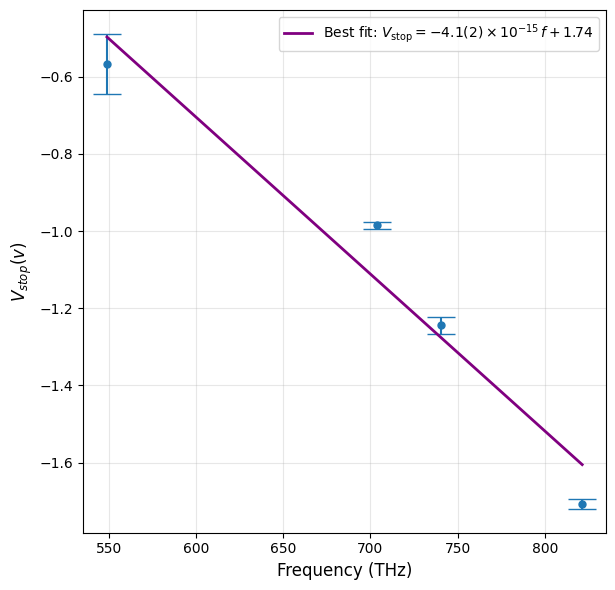
\includegraphics[width=0.8 \linewidth]{Freq2.png}
    \caption{Stopping voltage vs frequency scatter plot with slope h/e.}
    \label{Frequency}
\end{figure}

Fig. \ref{Frequency} shows the expected result: the stopping voltage decreases as the frequency increases. By rearranging eq. \ref{Vstop}, we find that Planck's constant ($h$) should equal the slope of the line ($V/f$) multiplied by the charge of the electrons ($e$). Similarly, the work function for the cathode can be obtained by multiplying the y-intercept by $e$. Using these methods, Planck's constant was estimated to be \SI{6.5(2)e-34}{\joule\second}, and the work function to be $2.78\text{eV}$. The accepted value for $h$ as reported by NIST is $\SI{6.626e-34}{\joule\second}$ \cite{Nist}, leaving a percent difference of only $1.92\%$ between the two values. Most common work functions generally fall between the values of $2eV$ and $5$ eV\cite{ChemPhys}. So while we don't know the exact work function of this apparatus's cathode, the experimental value still falls within the typical range.


For both data sets, the primary source of error was the voltage measurements. During data collection, the surrounding area was not entirely dark. This made it challenging to determine the exact cutoff for the stopping voltage, as ambient light induced a small but constant current. This problem became especially difficult for higher wavelengths such as $546 $ nm, and $577 $ nm (not included), where the current induced by the light source was not much larger than that of the ambient light. As a result, the current never truly reaches $0$ when the voltage is applied, leading to a larger margin of error. Lower frequencies most often induced a current value that was an order of magnitude higher than the ambient light. On that larger scale, the contributions of ambient light weren't nearly as noticeable. This would be why the uncertainty for wavelength $546 $ nm is so much larger than the rest.

\section{Conclusion}

This experiment aimed to demonstrate and confirm Einstein's theories about light using the photoelectric effect. By measuring the stopping voltage at various frequencies and light intensities, we established that, in the photoelectric effect, light behaves as particles. Some of the evidence gathered for this was that the stopping voltage depended on frequency and not intensity. This implies that the interactions between light and electrons are more individualized, with electrons absorbing only as much energy as a single photon can transfer. Einstein's theory was then further confirmed by the fact that Planck's constant could be calculated within 2\% of its actual value using equations consistent with particle theory. This work does not disprove wave theory as a whole but instead introduces the idea of wave-particle duality, in which the behavior of light is context-dependent. In some cases, like the double slit experiment, the wave model clearly makes the most sense. At the same time, other experiments, like the photoelectric effect, can only be explained by particle theory. 

\section*{Data Availability Statement}
A Jupyter notebook containing all the experimental data, data analysis, figure generation, and additional information on uncertainty analysis can be found in the supplemental materials. \footnote{See online article posting for access to supplemental material.}

\bibliography{apssamp}% Produces the bibliography via BibTeX.

\end{document}
%
% ****** End of file apssamp.tex ******
